% !TeX spellcheck = ru_RU
\documentclass[a4paper,12pt]{extarticle}
\usepackage[utf8x]{inputenc}
\usepackage[T1,T2A]{fontenc}
\usepackage[russian]{babel}
\usepackage{hyperref}
\usepackage{indentfirst}
\usepackage{listings}
\usepackage{color}
\usepackage{here}
\usepackage{array}
\usepackage{multirow}
\usepackage{graphicx}

\usepackage{caption}
\renewcommand{\lstlistingname}{Программа} % заголовок листингов кода

\bibliographystyle{ugost2008ls}

\usepackage{listings}
\lstset{ %
extendedchars=\true,
keepspaces=true,
language=C,						% choose the language of the code
basicstyle=\footnotesize,		% the size of the fonts that are used for the code
numbers=left,					% where to put the line-numbers
numberstyle=\footnotesize,		% the size of the fonts that are used for the line-numbers
stepnumber=1,					% the step between two line-numbers. If it is 1 each line will be numbered
numbersep=5pt,					% how far the line-numbers are from the code
backgroundcolor=\color{white},	% choose the background color. You must add \usepackage{color}
showspaces=false				% show spaces adding particular underscores
showstringspaces=false,			% underline spaces within strings
showtabs=false,					% show tabs within strings adding particular underscores
frame=single,           		% adds a frame around the code
tabsize=2,						% sets default tabsize to 2 spaces
captionpos=t,					% sets the caption-position to top
breaklines=true,				% sets automatic line breaking
breakatwhitespace=false,		% sets if automatic breaks should only happen at whitespace
escapeinside={\%*}{*)},			% if you want to add a comment within your code
postbreak=\raisebox{0ex}[0ex][0ex]{\ensuremath{\color{red}\hookrightarrow\space}},
texcl=true,
inputpath=listings,                     % директория с листингами
}

\usepackage[left=2cm,right=2cm,
top=2cm,bottom=2cm,bindingoffset=0cm]{geometry}

%% Нумерация картинок по секциям
\usepackage{chngcntr}
\counterwithin{figure}{section}
\counterwithin{table}{section}

%%Точки нумерации заголовков
\usepackage{titlesec}
\titlelabel{\thetitle.\quad}
\usepackage[dotinlabels]{titletoc}

%% Оформления подписи рисунка
\addto\captionsrussian{\renewcommand{\figurename}{Рисунок}}
\captionsetup[figure]{labelsep = period}

%% Подпись таблицы
\DeclareCaptionFormat{hfillstart}{\hfill#1#2#3\par}
\captionsetup[table]{format=hfillstart,labelsep=newline,justification=centering,skip=-10pt,textfont=bf}

%% Путь к каталогу с рисунками
\graphicspath{{fig/}}

\usepackage{minted}

\begin{document}	% начало документа

% Титульная страница
\begin{titlepage}	% начало титульной страницы

	\begin{center}		% выравнивание по центру

		\large Санкт-Петербургский политехнический университет Петра Великого\\
		\large Институт компьютерных наук и технологий \\
		\large Кафедра компьютерных систем и программных технологий\\[6cm]
		% название института, затем отступ 6см
		
		\huge Телекоммуникационные технологии\\[0.5cm] % название работы, затем отступ 0,5см
		\large Отчет по лабораторной работе №7\\[0.1cm]
		\large Помехоустойчивое кодирование\\[5cm]

	\end{center}


	\begin{flushright} % выравнивание по правому краю
		\begin{minipage}{0.25\textwidth} % врезка в половину ширины текста
			\begin{flushleft} % выровнять её содержимое по левому краю

				\large\textbf{Работу выполнил:}\\
				\large Графов Д.И.\\
				\large {Группа:} 33531/2\\
				
				\large \textbf{Преподаватель:}\\
				\large Богач Н.В.

			\end{flushleft}
		\end{minipage}
	\end{flushright}
	
	\vfill % заполнить всё доступное ниже пространство

	\begin{center}
	\large Санкт-Петербург\\
	\large \the\year % вывести дату
	\end{center} % закончить выравнивание по центру

\thispagestyle{empty} % не нумеровать страницу
\end{titlepage} % конец титульной страницы

\vfill % заполнить всё доступное ниже пространство


% Содержание
\setcounter{page}{2}
% Содержание
\renewcommand\contentsname{\centerline{Содержание}}
\tableofcontents
\newpage




\section{Цель работы}
\begin{itemize}
	\item Познакомиться со средствами генерации и визуализации простых сигналов.
	\item Получить представление о спектрах телекоммуникационных сигналов.
\end{itemize}

\section{Программа работы}
\begin{itemize}
	\item С помощью языка программирования Python и его библиотек
	промоделировать синусоидальный и прямоугольный сигналы с различными параметрами. Получить их спектры. Вывести на график.
	\item \begin{itemize}
		\item Для сигналов, построенных в лабораторной работе №1, выполните расчет преобразования Фурье. Перечислите свойства преобразования Фурье.
		\item С помощью функции корреляции найдите позицию синхропосылки [101] в сигнале [0001010111000010]. Получите пакет данных, если известно, что его длина составляет 8 бит без учета синхропосылки. Вычислите корреляцию прямым методом, воспользуйтесь алгоритмом быстрой корреляции, сравните время работы обоих алгоритмов.
	\end{itemize}
\end{itemize}

\section{Теоретическая информация}
\subsection{Python и используемые библиотеки}
Среди множества библиотек Python выделим основные, используемые для математических расчётов и визуализации.
\begin{itemize}
	\item \textbf{NumPy} -- это open-source модуль для Python, который предоставляет общие математические и числовые операции в виде пре-скомпилированных, быстрых функций. Они объединяются в высокоуровневые пакеты. Они обеспечивают функционал, который можно сравнить с функционалом MatLab. NumPy (Numeric Python) предоставляет базовые методы для манипуляции с большими массивами и матрицами. SciPy (Scientific Python) расширяет функционал numpy огромной коллекцией полезных алгоритмов, таких как минимизация, преобразование Фурье, регрессия, и другие прикладные математические техники.
	
	\item \textbf{Matplotlib} — библиотека на языке программирования Python для визуализации данных двумерной (2D) графикой (3D графика также поддерживается). Получаемые изображения могут быть использованы в качестве иллюстраций в публикация.
	
	Генерируемые в различных форматах изображения могут быть использованы в интерактивной графике, в научных публикациях, графическом интерфейсе пользователя, веб-приложениях, где требуется построение диаграмм (англ. plotting). В документации автор признаётся, что Matplotlib начинался с подражания графическим командам MATLAB, но является независимым от него проектом.
	
	Библиотека Matplotlib построена на принципах ООП, но имеет процедурный интерфейс pylab, который предоставляет аналоги команд MATLAB.
\end{itemize}

\subsection{Сигнал и его спектр}
\begin{itemize}
	\item \textit{Сигнал} - это физическое явление, служащее для передачи информации, которое может иметь различную природу. Должен также иметь различимые состояния (минимум 2), чтобы передавать информацию (например, наличие сигнала и его отсутствие).
	
	\item \textit{Спектр сигнала} - это результат разложения сигнала на более простые в базисе ортогональных функций. В качестве разложения обычно используются преобразование Фурье и другие.
	
	\begin{center}
		В радиотехнике в качестве базисных функций используют синусоидальные функции. Это объясняется рядом причин:
	\end{center}
	\item гармоническое колебание является единственной функцией времени, сохраняющей свою форму при прохождении колебания через линейную систему с постоянными параметрами, могут только изменяться амплитуда и фаза;
	\item для гармонических функций имеется математический аппарат комплексного анализа;
	\item гармоническое колебание легко реализуемо на практике. 
	
	\item Спектр сигнала $s(t)$ можно записать через преобразование Фурье (можно без коэффициента $ 1/{\sqrt {2\pi }}$) в виде:
	
	$ S(\omega )=\int_{-\infty }^{+\infty }s(t)e^{-i\omega t}dt $, где $\omega $ - угловая частота равная $ 2\pi f $.
	
	Спектр сигнала является комплексной величиной и представляется в виде: \\
	$ S(\omega )=A(\omega )e^{-i\phi (\omega )}$, где $A(\omega )$ - амплитудно-частотная характеристика сигнала, $\phi (\omega ) $ - фазо-частотная характеристика сигнала.
	\end {itemize}

\subsection{Свойства преобразования Фурье}
Перечислим некоторые свойства преобразования Фурье.
\begin{itemize}
	\item Преобразование Фурье является линейным оператором.
	\item Свойство временного сдвига: задержка сигнала во времени приводит к изменению фазы его спектральной плотности без изменения амплитуды.
	\item Преобразование Фурье свертки сигналов: спектральная плотность свертки двух сигналов равна произведению их спектральных плотностей.
	\item Преобразование Фурье произведения сигналов: преобразование Фурье произведения сигналов пропорционально свертке спектральных плотностей этих сигналов.
\end{itemize}

\newpage
\section{Ход выполнения работы}

\subsection{Лабораторная работа №1}
На языке python мной была написана программа, генерирующая синусоидальный и прямоугольный сигналы, а также отображающая их спектры.

\large {Листинг 1. main.py}
\inputminted[
frame=lines,
framesep=2mm,
baselinestretch=1.2,
fontsize=\footnotesize,
linenos
]{python}{../../lab1/src/main.py}

\large {Результат работы}
\begin{figure}[H]
	\begin{center}
		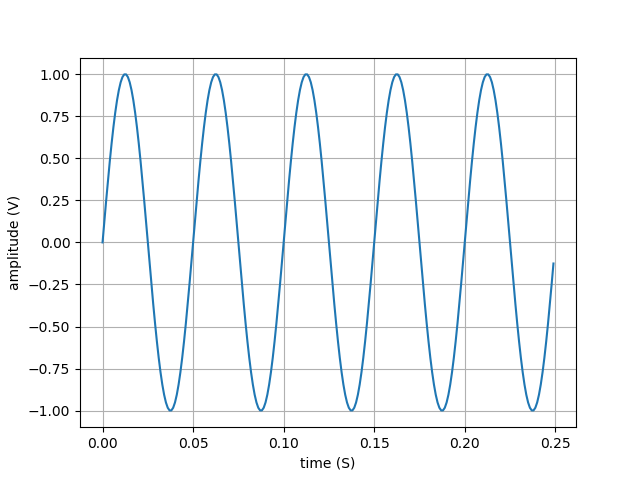
\includegraphics[scale=0.7]{../../lab1/out/sine_time.png}
		\caption{Синусоидальный сигнал} 
		\label{pic:sine_time} % название для ссылок внутри кода
	\end{center}
\end{figure}

\begin{figure}[H]
	\begin{center}
		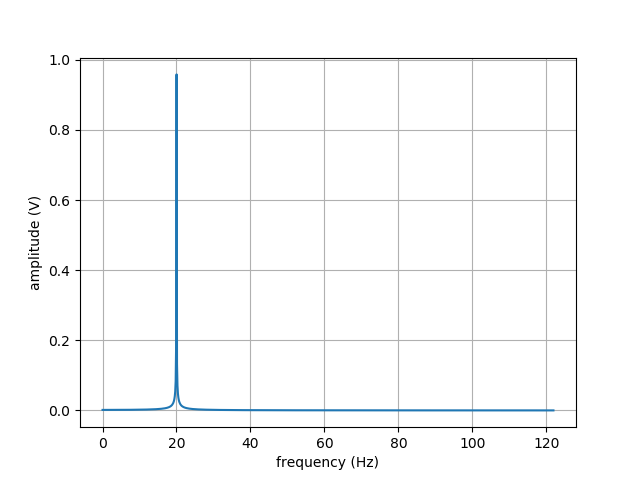
\includegraphics[scale=0.7]{../../lab1/out/sine_freq.png}
		\caption{Спектр синусоидального сигнала} 
		\label{pic:sine_freq} % название для ссылок внутри кода
	\end{center}
\end{figure}

\begin{figure}[H]
	\begin{center}
		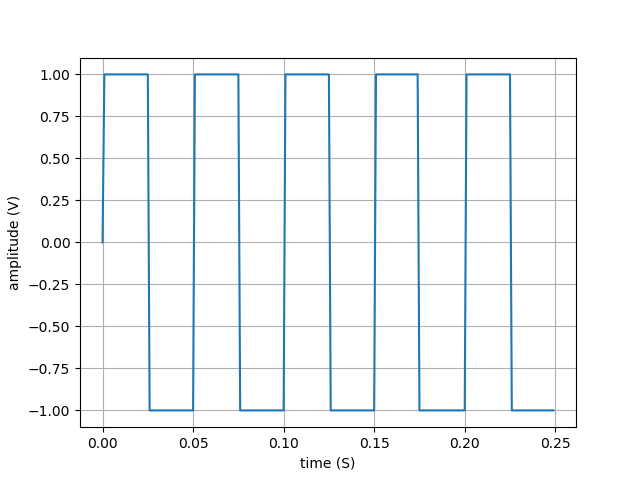
\includegraphics[scale=0.7]{../../lab1/out/square_time.png}
		\caption{Прямоугольный сигнал} 
		\label{pic:square_time} % название для ссылок внутри кода
	\end{center}
\end{figure}

\begin{figure}[H]
	\begin{center}
		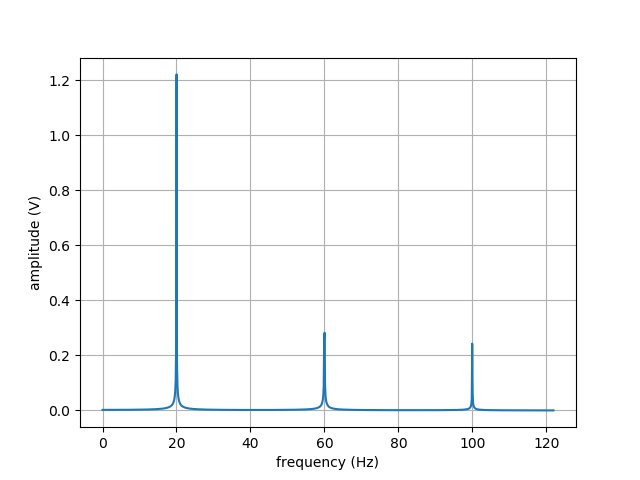
\includegraphics[scale=0.7]{../../lab1/out/square_freq.png}
		\caption{Спектр прямоугольного сигнала} 
		\label{pic:square_freq} % название для ссылок внутри кода
	\end{center}
\end{figure}

\newpage
\subsection{Лабораторная работа №2}
\subsubsection{Расчёт преобразования Фурье}
Вспомогательные формулы:
\begin{itemize}
	\item $ \sin(\omega_0 t) = \frac{e^{i \omega_0 t} - e^{-i \omega_0 t}}{2 i} $
	\item Дельта-функция: $ \delta(\omega) = \frac{1}{2 \pi} \int_\infty^\infty e^{i \omega t} dt $
	\item $ \delta(t) = \delta(-t) $
\end{itemize}

$F(\omega) = \frac{1}{\sqrt{2 \pi}} \int_\infty^\infty f(t) e^{-i \omega t} dt = 
\frac{1}{\sqrt{2 \pi}} \int_\infty^\infty \sin(\omega_0 t) e^{-i \omega t} dt = 
\frac{1}{\sqrt{2 \pi}} \int_\infty^\infty \frac{e^{i \omega_0 t} - e^{-i \omega_0 t}}{2 i} e^{-i \omega t} dt = 
\frac{\sqrt{2 \pi}}{2 \pi 2 i} \int_\infty^\infty (e ^ {i t (\omega - \omega_0)} - e^{-it(\omega - \omega_0)}) dt = 
\frac{\sqrt{2 \pi}}{2 i} (\delta(\omega - \omega_0) - \delta(\omega + \omega_0) $

\subsubsection{Программа}
\large {Листинг 2. main.py}
\inputminted[
frame=lines,
framesep=2mm,
baselinestretch=1.2,
fontsize=\footnotesize,
linenos
]{python}{../src/main.py}

\large {Результат работы}

\begin{lstlisting}
	Direct method:
	--- 2.5033950805664062e-05 seconds ---
	FFT method:
	--- 0.0203402042388916 seconds ---
	Correlations using direct method: [0 1 0 2 0 2 1 2 1 1 0 0 0 1 0]
	Correlations using FFT method   : [0 1 0 2 0 2 1 2 1 1 0 0 0 1 0]
	Position with direct correlation: 3
	Position with FFT correlation   : 3
	Package:  [0 1 1 1 0 0 0 0]
\end{lstlisting}

\begin{figure}[H]
	\begin{center}
		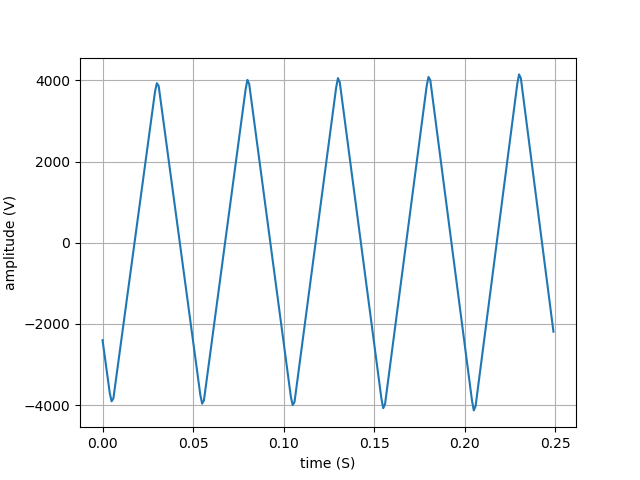
\includegraphics[scale=0.7]{../out/triangle_time.png}
		\caption{Треугольный сигнал} 
		\label{pic:trinagle_time} % название для ссылок внутри кода
	\end{center}
\end{figure}

\begin{figure}[H]
	\begin{center}
		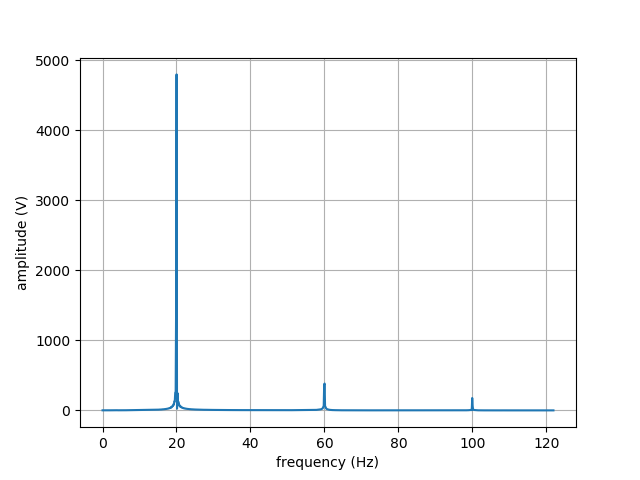
\includegraphics[scale=0.7]{../out/triangle_freq.png}
		\caption{Спектр треугольного сигнала} 
		\label{pic:trinagle_freq} % название для ссылок внутри кода
	\end{center}
\end{figure}


\newpage
\section{Выводы}
В данных лабораторных работах (1 и 2) мной были промоделированы синусоидальный и прямоугольные сигналы, получены их спектры.

Был проведён расчёт преобразования Фурье для синусоидального сигнала. Были перечислены свойства данного преобразования.

С помощью функции корреляции была найдена позиция синхропосылки в сигнале, был получен пакет данных. Корреляция была вычислена прямым методом, и методом быстрой корреляции.

В ходе выполнения работы я познакомился со средствами генерации сигналов, их визуализации. Также было получено представление о спектрах телекоммуникационных сигналов.
\end{document}
